%\documentclass[12pt,handout]{beamer}
\documentclass{beamer}
\usepackage[ngerman]{babel}
\usepackage[utf8]{inputenc}
\usepackage{amsmath}
\usepackage{amssymb}
\usepackage{listings} 
\usepackage{mathtools}
\usepackage{ulem}
\usetheme{Boadilla}

\parskip 10pt


\begin{document}
\title{Sortierverfahren}   
\author{Informatik} 
\date{ } 


\lstset{language=Python, tabsize=4, showstringspaces=false,basicstyle=\footnotesize,mathescape=true}
\lstset{literate=%
  {Ö}{{\"O}}1
  {Ä}{{\"A}}1
  {Ü}{{\"U}}1
  {ß}{{\ss}}1
  {ü}{{\"u}}1
  {ä}{{\"a}}1
  {ö}{{\"o}}1
}

\frame{\titlepage} 

%---
\begin{frame}[fragile]

Die unterschiedlichen Sortierverfahren eignen sich gut, um verschiedene Programmierstrategien
zu zeigen: \pause
\begin{itemize}
\item Eine \textit{Greedy} Strategie versucht durch \textit{gieriges} Vorgehen das jeweils kurzfristig bestmögliche zu erreichen. \pause
\item Bei \textit{Divide and Conquer} wird zunächst das gegebene Problem in Teilprobleme zerlegt, dann deren Lösung zur Gesamtlösung zusammengeführt. \pause 
\item \textit{Rekursive} Verfahren lösen die ursprüngliche Aufgabenstellung auf einer reduzierten Problemgröße mit demselben Lösungsansatz und konstruieren aus dieser Teillösung die Gesamtlösung.
\end{itemize}

Motivation fürs Sortieren: \pause
 Häufiges Suchen. Einmal Sortieren, dann jeweils $\log n$ Aufwand beim Suchen.
\end{frame}


%----
\begin{frame}[fragile]

Selection Sort 

\glqq Hole jeweils das kleinste Element nach vorne\grqq  

\begin{tabular}{lllllll}
15 & 23 & 4 & 42 & 8 & 16 \\ \pause
4 & 23 & 15 & 42 & 8 & 16 \\  
4 & 8 & 15 &  42 & 23 &  16  \\   
 4 & 8 & 15 & 16 & 23  &  42  \\ 
\end{tabular}
\end{frame}

%----
\begin{frame}[fragile]
\begin{lstlisting} 
def selection_sort(a):
    for i in range(len(a)-1):
        pos = i
        min = a[i]
        for j in range(i+1,len(a)):
            if a[j] < min:
                pos = j
                min = a[j]
        a[pos], a[i] = a[i], a[pos]
 \end{lstlisting} 
\end{frame}

%----
\begin{frame}[fragile]

Analyse für Selection Sort  

Wird der Algorithmus schneller, wenn die Daten schon sortiert sind? \pause Nein.

Anzahl Vergleiche bei den zwei ineinander geschachtelten for-Schleifen:  \pause

$(n-1) +  (n-2) + (n-3) + ... + 1 =  \frac{n \cdot (n-1)}{2} =\frac{n^2 - n}{2} \in  O(n^2)$ 

worst case  = best case  = average case: $O(n^2)$ 

Zusätzlicher Platzbedarf: \pause $O(1)$

Selection Sort ist ein Greedy-Algorithmus.

\end{frame}

%----
\section{Bubble Sort}
\begin{frame}[fragile]

Bubble Sort  = große Blasen steigen nach oben auf 

\glqq Vertausche jeweils unsortierte Nachbarn \grqq 

\begin{tabular}{cccccc}
15 & 23 & 4 & 42 & 8 & 16 \\ \pause
15 & 4 & 23 & 8 & 16 & 42 \\
4 & 15 & 8 & 16 & 23 & 42 \\ 
4 & 8 & 15 & 16 & 23 & 42 \\ 
\end{tabular}



\end{frame}


%----
\begin{frame}[fragile]
\begin{lstlisting} 
def bubble_sort(a):
    getauscht = True
    while getauscht:
        getauscht = False
        for i in range(len(a)-1):
            if a[i] > a[i+1]:
                a[i],a[i+1]=a[i+1],a[i]
                getauscht = True
\end{lstlisting} 
\end{frame}

%----
\begin{frame}[fragile]

Analyse von Bubble Sort 

Best case: \pause  $O(n)$ \\
Worst case: \pause (wenn die Folge ungekehrt sortiert ist) $O(n^2)$ \\
Average case: $O(n^2)$ 

Weitere Verbesserungen möglich: Shaker Sort, aber es bleibt bei  $O(n^2)$. 
Grund: die Austauschpositionen liegen zu nahe beieinander.

Zusätzlicher Platzbedarf: \pause $O(1)$

Bubble Sort ist ein Greedy-Algorithmus.
\end{frame}

%----
\section{MergSort}
\begin{frame}[fragile]
Mergesort

Idee (rekursiv formuliert): 

~~~~ - Sortiere die vordere Hälfte der Folge \\ 
~~~~ - Sortiere die hintere Hälfte der Folge \\ 
~~~~ - Mische die beiden sortierten Folgen zu einer sortierten Folge \pause

Die Vorgehensweise wird \textit{Divide and Conquer} genannt. Das ursprüngliche Problem wird in 
unabhängige Teilprobleme zerlegt, danach werden die Teillösungen zur Gesamtlösung zusammengefügt. \pause

7~~ 13 ~~ 15 ~~ 18   ~~~~  ~~~~2 ~~  4 ~~ 19 ~~ 22  \pause

2 ~~ 4 ~~ 7 ~~ 13 ~~ 15 ~~ 18 ~~19 ~~ 22  
\end{frame}

%----
\begin{frame}[fragile]

Die Hilfsfunktion \textit{merge} zum Mischen der sortierten Teilfolgen:  
\begin{lstlisting} 
def merge(a, b):
    i = j = 0
    c=[]
    while i < len(a) and j < len(b):
        if a[i] < b[j]:
            c.append(a[i])
            i+=1
        else:
            c.append(b[j])
            j+=1
    c+=a[i:]+b[j:]  
    return c
\end{lstlisting} 
\end{frame}


%----
\begin{frame}[fragile]

\begin{lstlisting} 
def merge_sort(a):
    if len(a) <= 1: return a
    halb = len(a)//2
    b = a[:halb]
    c = a[halb:]
    return merge(merge_sort(b),merge_sort(c))
\end{lstlisting} 
\end{frame}





%----
\begin{frame}[fragile]

Die Liste \texttt{a = [17,3,23,4,1,9,11]} wird mit Merge Sort sortiert. \\
a. Wieviel mal wird \texttt{merge} aufgerufen?  \\
b. Wieviel mal wird \texttt{mergeSort} aufgerufen? \\
c .Bei jedem Aufruf von \texttt{merge} wird eine Liste zurückgegeben.
Notiere die Listen in der Reihenfolge, in der sie zurückgegeben werden.  \pause
 
a. 6   ~~~ b. 13
\begin{lstlisting}
3 23
3 17 23
1 4
9 11
1 4 9 11
1 3 4 9 11 17 23
\end{lstlisting}  

\end{frame}

%----
\begin{frame}[fragile]

Analyse von MergeSort\pause

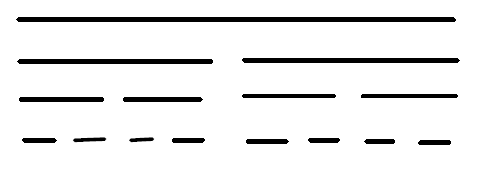
\includegraphics[scale=0.6]{mergesort1.png} 

Anzahl Ebenen: $\log n$ \\ \pause
Aufwand pro Ebene: \pause $O(n)  \Rightarrow$ Laufzeit:  \pause  $O(n \cdot \log n)$  

zusätzlicher Platzbedarf: \pause $O(n)$

\end{frame}

%----
\begin{frame}[fragile]
QuickSort 

Idee: teile die Folge in eine elementweise kleinere und eine elementweise größere Hälfte und sortiere diese
nach demselben Verfahren. 

\texttt{15 26 22 18 16 28 9 38 8} \pause

\begin{lstlisting}
15 26 22 18 16 28 9 38 8 -  0-8, pivot=16
15 8 9 16 18 28 22 38 26 -  0-3, pivot= 8
8 15 9 16 18 28 22 38 26 -  1-3, pivot= 9
8 9 15 16 18 28 22 38 26 -  2-3, pivot=15
8 9 15 16 18 28 22 38 26 -  4-8, pivot=22
8 9 15 16 18 22 28 38 26 -  4-5, pivot=18
8 9 15 16 18 22 28 38 26 -  6-8, pivot=38
8 9 15 16 18 22 28 26 38 -  6-7, pivot=28
\end{lstlisting}

\end{frame}


\begin{frame}[fragile]

Analyse von QuickSort

best case: \pause Pivot-Element so, dass ungefähr gleich große Hälften entstehen.  
Dann gibt es $\log n$ Rekursionsebenen. 
Pro Ebene muss einmal durchs Array gelaufen werden,  also insgesamt:  $O(n \cdot \log n)$

worst case: \pause Pivot-Element so, dass ein Teil immer nur aus einem Element besteht. \\ 
$n + (n-1) + (n-2) + (n-3) + ... 1 \in O(n^2)$

average case: $O(n \cdot \log n)$. 

Zusätzlicher Platz: \pause $O(\log n)$ \\
(nicht $O(1)$ denn in jeder der Rekursionsebenen benötigt man eine konstante Anzahl Variablen)

\end{frame}

%----
\begin{frame}[fragile]
\begin{lstlisting} 
def quick_sort(a,unten=0,oben=None):
    if oben is None: oben = len(a)-1
    i , j = unten, oben
    mitte = (unten +  oben) // 2
    pivot = a[mitte]
    while i <= j:
        while a[i] < pivot: i+=1
        while a[j] > pivot: j-=1
        if i <= j:
            a[i],a[j]=a[j],a[i]
            i, j = i+1, j-1
    if unten < j: quick_sort(a,unten,j)
    if i < oben: quick_sort(a,i,oben)
\end{lstlisting} 
\end{frame}

\begin{frame}[fragile]

Beispiel dafür, dass die Abfrage \texttt{if i <= j} notwendig ist: [2, 4, 3, 1]  \pause
\begin{lstlisting} 
2 4 3 1  -$\pause$ 0-3, pivot=4
2 1 4 3  - 0-1, pivot=2
1 2 4 3   # falsches Resultat ohne die Abfrage
\end{lstlisting}  \pause

Tausch mit sich selbst
\begin{lstlisting} 
3 2 1 4  -$\pause$ 0-3, pivot=2
1 2 3 4  - 2-3, pivot=3
1 2 3 4
\end{lstlisting} 
\end{frame}


 \end{document}